\section{Code design and implementation}
\label{sec:code}
\begin{figure}
  \begin{center}
    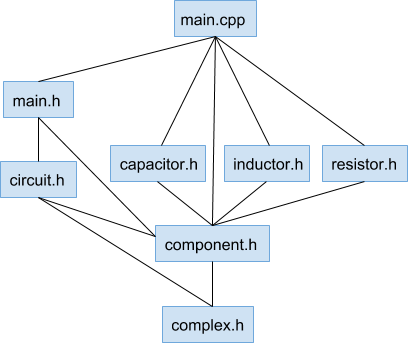
\includegraphics[width=.5\textwidth]{hierarchy}
  \end{center}
  \caption{The hierarchy of header files showing the main file at the top and the chain of its dependencies leading down.}
  \label{fig:hierarchy}
\end{figure}
In the design of this project, the code was split into seven header files, the hierarchical structure of which is shown in figure~\ref{fig:hierarchy}, which contained class definitions, function prototypes and a namespace definition while the implementation of the classes, the full functions and the \verb!main! function were separated into seven source files in line with the practice of abstraction, whereby the user is only exposed to the parts of the program which they need to actually use the program, and the details like the member data are hidden from them.

Splitting the code into several files makes it easier to reuse code, limits the \verb!#include! preprocessor directives to what is required only for the small piece of code in the file, and not for the entire program, reducing the risk of name clashes. Separating into different files can also reduce the compile time, as only the parts that have been changed need to be recompiled and the rest can just be linked again by the compiler.

Header guards were put in place to avoid header files being included multiple times. By using the preprocessor directives to define a unique constant for each header file, the compiler could check using a single if statement whether the header had already been included. This avoids compiler errors caused by apparent redefinitions of existing functions and other problems.

A custom complex class was used for dealing with complex numbers instead of using the standard library type definition. The class contained member data of the type double to store the real and imaginary parts and member functions including functions to return the complex conjugate, modulus and argument of a complex number, all of which were used in the calculation of the impedance and the phase difference.

For the components, an abstract base class \verb!Component! was created, from which three derived classes inherited: \verb!Resistor!, \verb!Capacitor! and \verb!Inductor!. The component class defined the functions that the three derived classes had in common -- for instance functions to access and modify the label of the components and a general constructor which was called by the derived classes. The component class had a pure virtual function \verb!get_impedance()! which was then defined in the derived classes and meant that polymorphic arrays could be created so that the derived classes would share a common interface. In this way the same function would carry out a different calculation depending on what type of object it was called on.

A circuit base class was created which was similar to the component base class in that it functions as a shared interface for the series and parallel derived classes. Again, the function to calculate the total impedance was left as a pure virtual function in the base class, to be defined in the correct way within the series and parallel classes. The series and parallel classes also each had specific functions to print out a circuit diagram in the correct layout for the circuit type. This was done using

The aim of the project was to be able to add components to a library of components which could be printed and the components stored in the library could be connected in specified groups to create circuits. The aim was to have a similar functionality for all circuits that had been made so far, so that circuits from the circuit library could be nested inside other circuits. This was acheived by making two polymorphic vectors of base class pointers -- one for components and the other for circuits. These polymorphic vectors were put inside the namespace \verb!libs! in \verb!main.h! so that it could be accessed from any function using the namespace and the binary scope operator (\verb!libs::!). If the libraries were used multiple times in the same function, \verb!using namespace libs! could be used once to remove the need to type the namespace and binary scope operator repeatedly within the relevant function.

To ensure that the label of components and circuits is always unique, static member data was used to keep track of the number of each type of component had been added so far

vectors iterators etc\\
smart pointers\\
lambdas\\
function template\\
static data\\
